\begin{figure}
    \centering
    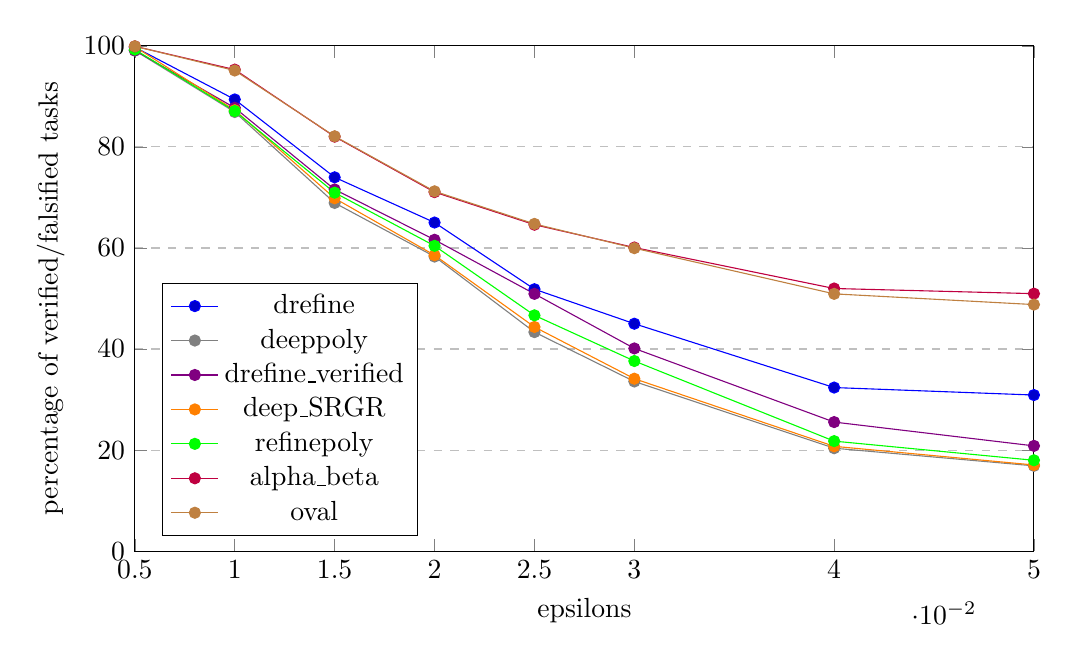
\begin{tikzpicture}
        \begin{axis}[
            xlabel={epsilons},
            ylabel={percentage of verified/falsified tasks},
            width=13cm,
            height=8cm,
            xmin=0.005, xmax=0.05,
            ymin=0, ymax=100,
            xtick={0.005,0.01,0.015,0.02,0.025,0.03,0.04,0.05},
            ytick={0,20,40,60,80,100},
            legend pos=south west,
            legend entries={drefine,deeppoly, drefine\_verified, deep\_SRGR, refinepoly, alpha\_beta, oval},
            ymajorgrids=true,
            grid style=dashed,
        ]
        \addplot+[
            color=blue,
            mark=*,
        ]
        coordinates {
            (0.005,99.72)(0.01,89.39)(0.015,73.98)(0.02,65.03)(0.025,51.84)(0.03,45.01)(0.04,32.38)(0.05,30.9)
        };

        \addplot[
            color=gray,
            mark=*,
        ]
        coordinates {
            (0.005,99.07)(0.01,86.9)(0.015,68.91)(0.02,58.3)(0.025,43.35)(0.03,33.58)(0.04,20.38)(0.05,16.89)
        };

        \addplot[
            color=violet,
            mark=*,
        ]
        coordinates {
            (0.005,99.07)(0.01,87.73)(0.015,71.58)(0.02,61.62)(0.025,50.92)(0.03,40.12)(0.04,25.55)(0.05,20.84)
        };

        \addplot[
            color=orange,
            mark=*,
        ]
        coordinates {
            (0.005,99.8)(0.01,87.26)(0.015,69.83)(0.02,58.57)(0.025,44.37)(0.03,34.13)(0.04,20.75)(0.05,17.06)
        };

        \addplot[
            color=green,
            mark=*,
        ]
        coordinates {
            (0.005,99.26)(0.01,87.08)(0.015,70.94)(0.02,60.42)(0.025,46.67)(0.03,37.63)(0.04,21.78)(0.05,17.99)
        };

        \addplot[
            color=purple,
            mark=*,
        ]
        coordinates {
            (0.005,99.9)(0.01,95.29)(0.015,82.02)(0.02,71.05)(0.025,64.60)(0.03,60.09)(0.04,51.98)(0.05,50.96)
        };

        \addplot[
            color=brown,
            mark=*,
        ]
        coordinates {
            (0.005,99.9)(0.01,95.11)(0.015,82.1)(0.02,71.21)(0.025,64.76)(0.03,59.96)(0.04,50.92)(0.05,48.8)
        };


        \end{axis}

    \end{tikzpicture}
    \caption{Epsilon wise comparison with related techniques}
    \label{res:ep:milp_with_milp}
\end{figure}